\chapter{M\'odulo de Facturaci\'on}

\section{Descripci\'on General}

El m\'odulo de facturaci\'on gestiona la creaci\'on de facturas con IVA,
partidas din\'amicas y transiciones de estado. Incluye tambi\'en la gesti\'on
de productos y proveedores como parte del ciclo de facturaci\'on.

\section{Generaci\'on de N\'umero de Factura}

Los n\'umeros de factura siguen el formato \texttt{INV-XXXXXX}:

\begin{lstlisting}[style=typescript, caption=Generacion secuencial de numero de factura]
async function nextInvoiceNumber(): Promise<string> {
  const last = await db
    .select({ num: schema.invoices.invoiceNumber })
    .from(schema.invoices)
    .orderBy(desc(schema.invoices.invoiceNumber))
    .limit(1)
    .then((r) => r[0]?.num);

  const nextNum = last
    ? String(Number(last.replace('INV-', '')) + 1)
        .padStart(6, '0')
    : '000001';

  return `INV-${nextNum}`;
}
\end{lstlisting}

\section{C\'alculo de IVA y Totales}

\begin{lstlisting}[style=typescript, caption={Calculo de subtotal, IVA 16\% y total}]
const subtotal = data.items.reduce(
  (sum, item) => sum + Number(item.unitPrice) * item.quantity,
  0,
);
const tax = Math.round(subtotal * 0.16 * 100) / 100;
const total = subtotal + tax;
\end{lstlisting}

La tasa de IVA es fija del 16\%, aplicada autom\'aticamente sobre el subtotal.

\section{Creaci\'on de Factura con Partidas}

\begin{lstlisting}[style=typescript, caption=createInvoice - Insercion de factura y partidas]
export async function createInvoice(data: InvoiceInput) {
  const clinicId = await getCurrentClinicId();
  const invoiceNumber = await nextInvoiceNumber();

  const subtotal = data.items.reduce(
    (sum, item) => sum + Number(item.unitPrice) * item.quantity, 0);
  const tax = Math.round(subtotal * 0.16 * 100) / 100;
  const total = subtotal + tax;

  // Inserta la factura
  await db.insert(schema.invoices).values({
    clinicId, clientId: data.clientId,
    appointmentId: data.appointmentId || null,
    invoiceNumber, subtotal: String(subtotal),
    tax: String(tax), total: String(total),
    status: 'draft', notes: data.notes || null,
  });

  // Obtiene el ID de la factura recien creada
  const invoice = await db
    .select({ id: schema.invoices.id })
    .from(schema.invoices)
    .where(eq(schema.invoices.invoiceNumber, invoiceNumber))
    .then((r) => r[0]);

  // Inserta las partidas en bulk
  if (invoice && data.items.length > 0) {
    await db.insert(schema.invoiceItems).values(
      data.items.map((item) => ({
        invoiceId: invoice.id,
        description: item.description,
        quantity: item.quantity,
        unitPrice: item.unitPrice,
        total: String(Number(item.unitPrice) * item.quantity),
      })),
    );
  }

  // Notificacion
  await notifyNewInvoice({ ... });

  revalidatePath('/invoices');
  return invoice?.id;
}
\end{lstlisting}

\section{Transiciones de Estado}

Las facturas siguen el ciclo de vida:

\begin{verbatim}
draft --> issued --> paid
  |           |
  +--> cancelled
\end{verbatim}

\begin{itemize}[leftmargin=*]
    \item \textbf{draft:} Borrador, editable.
    \item \textbf{issued:} Emitida, no modificable.
    \item \textbf{paid:} Pagada, estado terminal.
    \item \textbf{cancelled:} Cancelada, estado terminal.
\end{itemize}

\section{P\'aginas}

\subsection{Listado de Facturas (/invoices)}

\begin{itemize}[leftmargin=*]
    \item Tabla con columnas: n\'umero, cliente, subtotal, IVA, total, estado.
    \item Colores sem\'anticos por estado (verde=paid, \'ambar=draft, etc.).
    \item Acciones r\'apidas: Emitir, Pagar, Cancelar.
\end{itemize}

\subsection{Creaci\'on (/invoices/new)}

\begin{itemize}[leftmargin=*]
    \item Selector de cliente (carga desde API).
    \item Cita opcional asociada.
    \item Conceptos din\'amicos: botones ``Agregar concepto'' y ``Eliminar''.
    \item C\'alculo autom\'atico de subtotal, IVA y total en tiempo real.
\end{itemize}

\subsection{Detalle (/invoices/[id])}

\begin{itemize}[leftmargin=*]
    \item Informaci\'on completa de la factura.
    \item Lista de partidas con c\'alculos.
    \item Acciones seg\'un estado actual.
    \item Bot\'on para descargar PDF de la factura.
\end{itemize}

\begin{figure}[H]
    \centering
    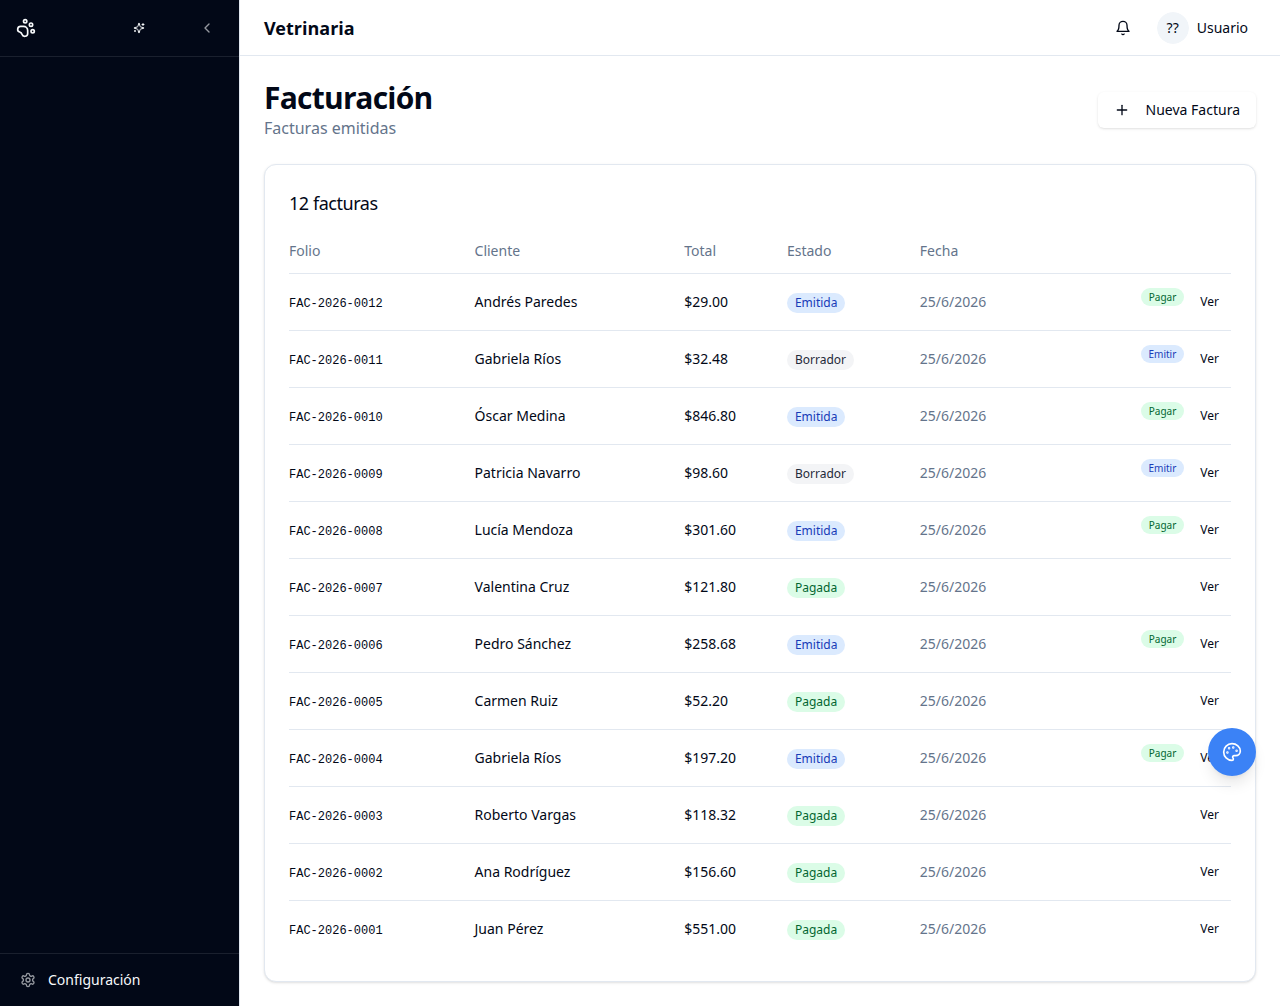
\includegraphics[width=\textwidth]{img/vet-invoices.png}
    \caption{Listado de facturas con estados y montos}
    \label{fig:facturas}
\end{figure}

\begin{figure}[H]
    \centering
    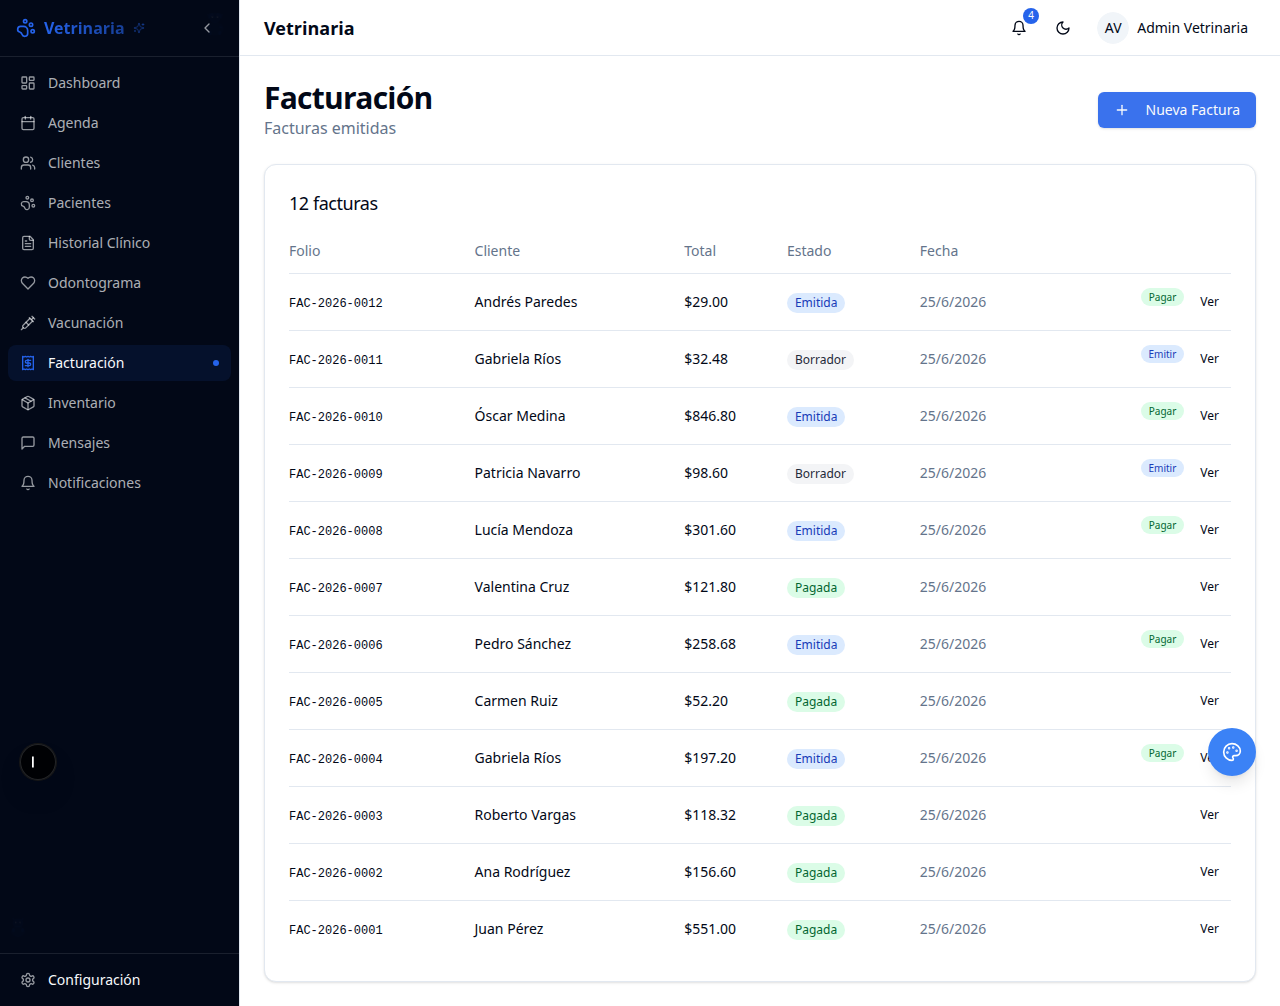
\includegraphics[width=0.8\textwidth]{img/vet-invoice-detail.png}
    \caption{Detalle de factura con boton de descarga PDF}
    \label{fig:factura-detalle}
\end{figure}

\section{Generaci\'on de PDF de Factura}

El sistema incluye un generador de PDF para facturas, accesible desde el
bot\'on ``PDF'' en la p\'agina de detalle de cada factura.

\subsection{API Route}

La descarga se realiza mediante una API Route de Next.js en
\texttt{/api/invoices/[id]/pdf}:

\begin{lstlisting}[style=typescript, caption=API Route de generacion de PDF]
export async function GET(
  _request: Request,
  { params }: { params: Promise<{ id: string }> },
) {
  const session = await auth();
  if (!session?.user) {
    return new NextResponse('Unauthorized', { status: 401 });
  }

  const { id } = await params;
  const invoiceId = Number(id);

  // Obtiene la factura con datos del cliente
  const invoice = await db
    .select({ ... })
    .from(schema.invoices)
    .innerJoin(schema.clients,
      eq(schema.invoices.clientId, schema.clients.id))
    .where(eq(schema.invoices.id, invoiceId))
    .then((r) => r[0] ?? null);

  if (!invoice) {
    return new NextResponse('NotFound', { status: 404 });
  }

  // Verifica pertenencia a la clinica
  if (invoice.clinicId !== session.user.clinicId
      && session.user.role !== 'super_admin') {
    return new NextResponse('Forbidden', { status: 403 });
  }

  // Obtiene datos de la clinica y partidas
  const clinic = await db.select()
    .from(schema.clinics)
    .where(eq(schema.clinics.id, invoice.clinicId))
    .then((r) => r[0] ?? null);

  const items = await db.select()
    .from(schema.invoiceItems)
    .where(eq(schema.invoiceItems.invoiceId, invoiceId));

  // Genera el PDF con pdfkit
  const pdfBuffer = await generateInvoicePdf(
    invoice, clinic, items);

  return new NextResponse(pdfBuffer, {
    headers: {
      'Content-Type': 'application/pdf',
      'Content-Disposition':
        `attachment; filename="factura-${invoice.invoiceNumber}.pdf"`,
    },
  });
}
\end{lstlisting}

\subsection{Diseno del PDF con pdfkit}

La funci\'on \texttt{generateInvoicePdf} utiliza la librer\'{\i}a
\textbf{pdfkit} para crear un documento PDF profesional con los siguientes
elementos:

\begin{itemize}[leftmargin=*]
    \item \textbf{Encabezado:} Nombre de la cl\'{\i}nica, direcci\'on,
          tel\'efono y correo electr\'onico.
    \item \textbf{Informaci\'on de factura:} N\'umero \'unico, fecha de
          emisi\'on y estado (Borrador, Emitida, Pagada, Cancelada) con
          color sem\'antico.
    \item \textbf{Datos del cliente:} Nombre, tel\'efono y correo.
    \item \textbf{Tabla de partidas:} Descripci\'on, cantidad, precio
          unitario y total, con filas alternadas de color.
    \item \textbf{Totales:} Subtotal, IVA (16\%) y total general.
    \item \textbf{Notas:} Notas adicionales de la factura.
    \item \textbf{Pie de p\'agina:} Mensaje de factura generada
          electr\'onicamente.
\end{itemize}

\begin{lstlisting}[style=typescript, caption=Funcion generateInvoicePdf con pdfkit]
async function generateInvoicePdf(invoice, clinic, items) {
  return new Promise((resolve, reject) => {
    const doc = new PDFDocument({ margin: 50 });
    const chunks: Buffer[] = [];
    doc.on('data', (chunk) => chunks.push(chunk));
    doc.on('end', () => resolve(Buffer.concat(chunks)));
    doc.on('error', reject);

    // Encabezado: nombre de la clinica
    doc.fontSize(22).font('Helvetica-Bold')
       .text('FACTURA', 50, 50);
    doc.fontSize(18).font('Helvetica-Bold')
       .text(clinicName, 50, 88);

    // Numero de factura y fecha (lado derecho)
    doc.fontSize(16).font('Helvetica-Bold')
       .text(invoiceNumber, rightX, 64, { align: 'right' });

    // Tabla de partidas con cabecero oscuro
    doc.rect(50, tableTop, pageWidth, 20).fill('#1f2937');
    doc.fillColor('#fff').font('Helvetica-Bold').fontSize(9);
    doc.text('DESCRIPCION', colX[0] + 5, tableTop + 5);
    doc.text('CANT.', colX[2] + 5, rowY + 5,
             { width: 70, align: 'right' });
    doc.text('PRECIO', colX[3] + 5, rowY + 5,
             { width: 70, align: 'right' });
    doc.text('TOTAL', colX[4] + 5, rowY + 5,
             { width: 70, align: 'right' });

    // Filas con colores alternados
    for (const [i, item] of items.entries()) {
      if (i % 2 === 0) {
        doc.rect(50, rowY, pageWidth, 22).fill('#f9fafb');
      }
      doc.fillColor('#333').font('Helvetica').fontSize(9);
      doc.text(item.description, colX[0] + 5, rowY + 5);
      doc.text(String(item.quantity), colX[2] + 5, rowY + 5,
               { align: 'right' });
      doc.text(`$${Number(item.unitPrice).toFixed(2)}`,
               colX[3] + 5, rowY + 5, { align: 'right' });
      doc.text(`$${Number(item.total).toFixed(2)}`,
               colX[4] + 5, rowY + 5, { align: 'right' });
      rowY += 22;
    }

    // Totales: Subtotal, IVA 16%, Total
    doc.text(`Subtotal: $${subtotal}`, rightX, totalsY,
             { align: 'right' });
    doc.text(`IVA (16%): $${tax}`, rightX, totalsY + 18,
             { align: 'right' });
    doc.text(`TOTAL: $${total}`, rightX, totalsY + 46,
             { align: 'right' });

    doc.end();
  });
}
\end{lstlisting}

\subsection{Seguridad}

\begin{itemize}[leftmargin=*]
    \item La API Route verifica la sesi\'on del usuario antes de generar
          el PDF.
    \item Valida que la factura pertenezca a la cl\'{\i}nica del usuario
          autenticado (aislamiento multi-tenant).
    \item Los super\_admins pueden descargar facturas de cualquier
          cl\'{\i}nica.
    \item El archivo se sirve como descarga (Content-Disposition:
          attachment) para evitar visualizaci\'on directa en el navegador.
\end{itemize}

\section{Productos e Inventario}

El m\'odulo de productos (\texttt{/inventory}) gestiona el cat\'alogo:

\begin{itemize}[leftmargin=*]
    \item \textbf{Tipos:} medication, supply, food, service.
    \item \textbf{Stock:} Cantidad actual y punto de reorden.
    \item \textbf{Alertas:} Visual cuando stock $<$ reorderPoint.
    \item Precio de venta y precio de costo.
\end{itemize}

\section{Proveedores}

El m\'odulo de proveedores (\texttt{/suppliers}) gestiona:

\begin{itemize}[leftmargin=*]
    \item Nombre, contacto, email, tel\'efono, direcci\'on.
    \item Vista en tarjetas con grid responsivo.
\end{itemize}
